% \documentclass[UTF8,oneside]{ctexbook}
% \usepackage{pgfplots}
% \usepackage{caption}

% \usepackage{tikz}
% \usetikzlibrary{backgrounds}
% \usetikzlibrary{arrows}
% \usetikzlibrary{shapes,shapes.geometric,shapes.misc}

% \begin{document}

% \begin{figure}[!h]
% \centering
% \begin{tikzpicture}[
%     x=0.75pt,y=0.75pt,
%     yscale=-1,xscale=1,
%     font = \sffamily\Large,
%     every path/.append style ={line width = 0.8pt,},
% ]
    
%     % 矩形
%     \draw [
%         fill = {rgb, 255:red, 155; green, 155; blue, 155 },
%         fill opacity=0.3 
%     ] (42.67,94) -- (99.33,94) -- (99.33,208.68) -- (42.67,208.68) -- cycle ;
%     \draw [
%         fill = {rgb, 255:red, 0; green, 0; blue, 0 },
%         fill opacity=1 
%     ] (42.67,94) -- (99.33,94) -- (99.33,104.32) -- (42.67,104.32) -- cycle ;
    
%     \draw [
%         fill={rgb, 255:red, 155; green, 155; blue, 155 },
%         fill opacity=0.3 
%     ] (162,163.32) -- (349.65,163.32) -- (349.65,207.32) -- (162,207.32) -- cycle ;
%     \draw [
%         fill={rgb, 255:red, 0; green, 0; blue, 0 },
%         fill opacity=1 
%     ] (162,173.32) -- (349.65,173.32) -- (349.65,163.32) -- (162,163.32) -- cycle ;
    
%     % 箭头
%     \draw (129.65,63.23) -- (78.46,87.29) ;
%     \draw [shift={(76.65,88.14)}, rotate = 334.83] [color={rgb, 255:red, 0; green, 0; blue, 0 }  ][line width=0.75]    (10.93,-3.29) .. controls (6.95,-1.4) and (3.31,-0.3) .. (0,0) .. controls (3.31,0.3) and (6.95,1.4) .. (10.93,3.29)   ;
%     \draw (144.65,63.23) -- (196.65,153.4) ;
%     \draw [shift={(197.65,155.14)}, rotate = 240.03] [color={rgb, 255:red, 0; green, 0; blue, 0 }  ][line width=0.75]    (10.93,-3.29) .. controls (6.95,-1.4) and (3.31,-0.3) .. (0,0) .. controls (3.31,0.3) and (6.95,1.4) .. (10.93,3.29)   ;
%     \draw (264.65,100.23) -- (72.26,150.83) ;
%     \draw [shift={(70.33,151.34)}, rotate = 345.26] [color={rgb, 255:red, 0; green, 0; blue, 0 }  ][line width=0.75]    (10.93,-3.29) .. controls (6.95,-1.4) and (3.31,-0.3) .. (0,0) .. controls (3.31,0.3) and (6.95,1.4) .. (10.93,3.29)   ;
%     \draw (284.65,102.23) -- (284.65,189.14) ;
%     \draw [shift={(284.65,191.14)}, rotate = 270] [color={rgb, 255:red, 0; green, 0; blue, 0 }  ][line width=0.75]    (10.93,-3.29) .. controls (6.95,-1.4) and (3.31,-0.3) .. (0,0) .. controls (3.31,0.3) and (6.95,1.4) .. (10.93,3.29)   ;
    
%     % 文本
%     \draw (129,39.32)       node [align=center] { 
%         Interface\\(cost: less is better)
%     };
%     \draw (281,73.32)       node [align=center] {
%         Functionality\\(benefit: more is better)
%     };
%     \draw (71,229.32)       node [align=left] {Deep Module};
%     \draw (255.83,227.32)   node [align=left] {Shadow Module};
% \end{tikzpicture}
% \caption*{图 4.1}
% \label{fig:4-1}
% \end{figure}


\begin{figure}[!h]
% \ctikzfig{00012}
\centering

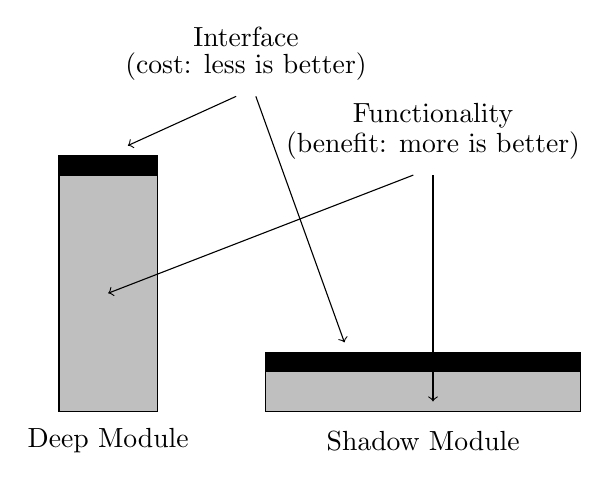
\begin{tikzpicture}[baseline=-0.25em,scale=0.5]
    % Node styles
    \tikzstyle{none}=[inner sep=0mm]
    \tikzstyle{medium box}=[fill=white, draw=black, shape=rectangle, minimum width=0.75cm, minimum height=1cm]
    \tikzstyle{gary box}=[fill={rgb,255: red,191; green,191; blue,191}, draw=black, shape=rectangle, minimum width=1.25cm, minimum height=3cm]
    \tikzstyle{black box}=[fill=black, draw=black, shape=rectangle, minimum width=1.25cm, minimum height=0.25cm]
    \tikzstyle{width gray box}=[fill={rgb,255: red,191; green,191; blue,191}, draw=black, shape=rectangle, minimum width=4cm, minimum height=0.75cm]
    \tikzstyle{width black box}=[fill=black, draw=black, shape=rectangle, minimum width=4cm, minimum height=0.25cm]
    % Edge styles
    \tikzstyle{arrow}=[->]
    \tikzstyle{every loop}=[]

    \node [style=gary box] (0) at (-4, 3.75) {};
    \node [style=black box] (1) at (-4, 7) {};
    \node [style=none] (4) at (-4, 0) {Deep Module};
    \node [style=none] (5) at (4, 0) {Shadow Module};
    \node [style=none] (6) at (-0.5, 10.25) {Interface};
    \node [style=none] (7) at (4.25, 8.25) {Functionality};
    \node [style=none] (8) at (-0.5, 9.5) {(cost: less is better)};
    \node [style=none] (9) at (4.25, 7.5) {(benefit: more is better)};
    \node [style=width gray box] (10) at (4, 1.5) {};
    \node [style=width black box] (11) at (4, 2) {};
    \node [style=none] (12) at (-0.75, 8.75) {};
    \node [style=none] (13) at (4.25, 6.75) {};
    \node [style=none] (14) at (-3.5, 7.5) {};
    \node [style=none] (15) at (-0.25, 8.75) {};
    \node [style=none] (16) at (3.75, 6.75) {};
    \node [style=none] (17) at (4.25, 1) {};
    \node [style=none] (18) at (-4, 3.75) {};
    \node [style=none] (19) at (2, 2.5) {};

    \draw [style=arrow] (13.center) to (17.center);
    \draw [style=arrow] (16.center) to (18.center);
    \draw [style=arrow] (12.center) to (14.center);
    \draw [style=arrow] (15.center) to (19.center);
\end{tikzpicture}

\caption*{图 4.1}
\label{fig:4-1}
\end{figure}

% \end{document}